\documentclass[aspectratio=169,10pt,t,xcolor={table}]{beamer}

% ─────────────────────────────────────────────────────────────────────────────
% EADD — JCSSE 2026 Slides v3
% Real matplotlib figures from experiments + refined UI/UX.
% Compile: pdflatex jcsse2026_slides_v3.tex (×2 for refs)
% Figures generated by: figures/make_figures.py
% ─────────────────────────────────────────────────────────────────────────────

\usepackage[T1]{fontenc}
\usepackage[scaled]{helvet}
\renewcommand{\familydefault}{\sfdefault}
\usepackage{lmodern}
\usepackage{amsmath,amssymb}
\usepackage{booktabs,array}
\usepackage{graphicx}
\usepackage{tikz}
\usetikzlibrary{arrows.meta,positioning,calc,shapes.geometric,backgrounds,fit,
                decorations.pathreplacing,patterns,shapes.symbols,shapes.misc}

% Locate figures dir
\graphicspath{{figures/}}

% ──────────────────── PALETTE ────────────────────
\definecolor{eaddDeep}{HTML}{0F3057}
\definecolor{eaddTeal}{HTML}{1B8A9C}
\definecolor{eaddCoral}{HTML}{E0625A}
\definecolor{eaddAmber}{HTML}{F4B942}
\definecolor{eaddLime}{HTML}{6FA84B}
\definecolor{eaddSlate}{HTML}{415A77}
\definecolor{eaddMist}{HTML}{F3F6FA}
\definecolor{eaddPaper}{HTML}{FAFBFD}
\definecolor{eaddInk}{HTML}{1B2A41}

% ──────────────────── BEAMER THEME ────────────────────
\setbeamercolor{normal text}{fg=eaddInk,bg=eaddPaper}
\setbeamercolor{background canvas}{bg=eaddPaper}
\setbeamercolor{alerted text}{fg=eaddCoral}
\setbeamercolor{example text}{fg=eaddTeal}
\setbeamercolor{frametitle}{fg=eaddDeep,bg=eaddPaper}
\setbeamercolor{title}{fg=white,bg=eaddDeep}
\setbeamercolor{block title}{fg=white,bg=eaddDeep}
\setbeamercolor{block body}{fg=eaddInk,bg=eaddMist}
\setbeamercolor{itemize item}{fg=eaddTeal}
\setbeamercolor{itemize subitem}{fg=eaddCoral}
\setbeamercolor{enumerate item}{fg=eaddCoral}
\setbeamercolor{section in toc}{fg=eaddDeep}
\setbeamercolor{structure}{fg=eaddDeep}

\setbeamerfont{frametitle}{series=\bfseries}
\setbeamerfont{title}{series=\bfseries}
\setbeamerfont{block title}{series=\bfseries}

\setbeamertemplate{navigation symbols}{}
\setbeamertemplate{itemize item}{\raisebox{0.18ex}{\tikz\fill[eaddTeal] (0,0) rectangle (1.2ex,1.2ex);}}
\setbeamertemplate{itemize subitem}{\textcolor{eaddCoral}{\textbf{--}}}
\setbeamertemplate{enumerate item}{\textcolor{eaddCoral}{\textbf{\insertenumlabel.}}}

% Frame title: small section tag + bold title + thin rule
\setbeamertemplate{frametitle}{%
  \nointerlineskip
  \vspace{0.55em}\hspace{1.2em}%
  \begin{tikzpicture}
    \node[anchor=south west,inner sep=0,text=eaddTeal,font=\fontsize{7}{8}\bfseries]
      at (0,0.74) {\eaddsec};
    \node[anchor=south west,inner sep=0,xshift=0,text=eaddDeep,font=\Large\bfseries]
      at (0,0.14) {\insertframetitle};
    \draw[eaddTeal,line width=1.2pt] (0,0) -- (1.6,0);
    \draw[eaddSlate!25,line width=0.4pt] (1.6,0) -- (\paperwidth-2.6cm,0);
  \end{tikzpicture}\vspace{-0.3em}%
}

% Footer: thin progress strip with right-aligned caption
\setbeamertemplate{footline}{%
  \leavevmode%
  \hspace{1.2em}%
  \begin{tikzpicture}
    \node[anchor=south east,text=eaddSlate,font=\fontsize{7}{8}\selectfont,inner sep=0]
      at (\paperwidth-2.4cm,0.30) {Begum et al. — Enhanced Adversarial Drift Detection \textbar{} JCSSE 2026 \textbar{} \insertframenumber\,/\,\inserttotalframenumber};
    \fill[eaddMist] (0,0) rectangle (\paperwidth-2.4cm,0.14);
    \pgfmathsetmacro{\progfrac}{\insertframenumber/\inserttotalframenumber}
    \fill[eaddTeal] (0,0) rectangle ({(\paperwidth-2.4cm)*\progfrac},0.14);
  \end{tikzpicture}\vspace{0.30em}%
}

% ──────────────────── HELPER MACROS ────────────────────
\newcommand{\statTile}[3]{%
  % #1 number, #2 label, #3 accent color
  \begin{tikzpicture}
    \fill[#3!10,rounded corners=4pt] (0,0) rectangle (3.05,1.85);
    \draw[#3,line width=0pt] (0,1.85) -- (0,0); % no border
    \fill[#3] (0,0) rectangle (0.10,1.85);
    \node[anchor=west,text=#3,font=\fontsize{22}{24}\bfseries]
      at (0.30,1.30) {#1};
    \node[anchor=west,text=eaddSlate,font=\scriptsize,align=left]
      at (0.30,0.55) {#2};
  \end{tikzpicture}%
}

\newcommand{\sectionDivider}[3]{%
  % #1 number, #2 title, #3 subtitle/tagline
  \begin{frame}[plain,noframenumbering]
    \begin{tikzpicture}[remember picture,overlay]
      \fill[eaddDeep] (current page.south west) rectangle (current page.north east);
      % accent stripe
      \fill[eaddTeal,opacity=0.18]
        ([yshift=0.5cm]current page.west) -- ([yshift=0.5cm,xshift=10cm]current page.west)
        -- ([yshift=2.4cm,xshift=10cm]current page.west)
        -- ([yshift=2.4cm]current page.west) -- cycle;
      % oversized section number
      \node[anchor=west,text=eaddTeal,font=\fontsize{90}{90}\bfseries,opacity=0.30]
        at ([xshift=1.4cm]current page.west) {#1};
      % small label
      \node[anchor=west,text=eaddAmber,font=\small\bfseries]
        at ([xshift=5.5cm,yshift=1.1cm]current page.west)
        {\rule[2pt]{0.5cm}{1.5pt}\hspace{0.3em}SECTION\,#1};
      % title
      \node[anchor=west,text=white,font=\Huge\bfseries]
        at ([xshift=5.5cm,yshift=0.2cm]current page.west) {#2};
      % subtitle
      \node[anchor=west,text=white!70,font=\normalsize\itshape]
        at ([xshift=5.5cm,yshift=-0.8cm]current page.west) {#3};
      % footer
      \node[anchor=south west,text=white!50,font=\scriptsize]
        at ([xshift=1.2cm,yshift=0.7cm]current page.south west)
        {EADD \textbar{} Enhanced Adversarial Drift Detection \textbar{} JCSSE 2026};
    \end{tikzpicture}
  \end{frame}
}

% Small section tracker (used by frame title)
\newcommand{\eaddsec}{}
\newcommand{\setsec}[1]{\renewcommand{\eaddsec}{#1}}

% ──────────────────── METADATA ────────────────────
\title{Enhanced Adversarial Drift Detection}
\author{Nusrat Begum \and Phaphontee Yamchote \and Chainarong Amornbunchornvej \and Thanapon Noraset}
\institute{Mahidol University \textbar{} NECTEC}
\date{JCSSE 2026 \textbar{} Bangkok \textbar{} June 24--27, 2026}

\begin{document}

% ════════════════════ TITLE ════════════════════
\setsec{}
\begin{frame}[plain,noframenumbering]
\begin{tikzpicture}[remember picture,overlay]
  % Background
  \fill[eaddDeep] (current page.south west) rectangle (current page.north east);
  % Diagonal accent band
  \fill[eaddTeal,opacity=0.55]
    (current page.north west) -- ([xshift=7.5cm]current page.north west)
    -- ([xshift=3.5cm]current page.south west) -- (current page.south west) -- cycle;
  % Subtle right-side rings
  \foreach \i in {0,1,2,3,4,5,6}{
    \draw[eaddAmber,opacity={0.10+0.02*\i},line width=0.6pt]
      ([xshift=-2cm-0.35*\i cm,yshift=-1.5cm-0.25*\i cm]current page.north east)
      circle ({1.0cm+0.4*\i cm});
  }
  \fill[eaddCoral] ([xshift=-3.5cm,yshift=-1.8cm]current page.north east) circle (0.20cm);
  \fill[eaddAmber] ([xshift=-2.4cm,yshift=-2.6cm]current page.north east) circle (0.10cm);

  % Eyebrow tag
  \node[anchor=west,text=eaddAmber,font=\fontsize{8}{10}\bfseries]
    at ([xshift=1.0cm,yshift=2.7cm]current page.west)
    {\rule[1.8pt]{0.7cm}{1.6pt}\hspace{0.4em}JCSSE 2026 \textbullet\ STREAMING ML \textbullet\ EXPLAINABLE AI};

  % Title
  \node[anchor=west,text=white,font=\fontsize{30}{34}\bfseries,align=left]
    at ([xshift=1.0cm,yshift=1.2cm]current page.west)
    {Enhanced Adversarial\\Drift Detection};
  \node[anchor=west,text=eaddAmber,font=\Large\itshape,align=left]
    at ([xshift=1.0cm,yshift=-0.6cm]current page.west)
    {for MLOps Feature Monitoring};

  % Authors
  \node[anchor=west,text=white,font=\small,align=left]
    at ([xshift=1.0cm,yshift=-1.8cm]current page.west)
    {\textbf{Nusrat Begum}$^{1}$\enspace\textbullet\enspace Phaphontee Yamchote$^{1}$\enspace\textbullet\enspace
     Chainarong Amornbunchornvej$^{2}$\enspace\textbullet\enspace Thanapon Noraset$^{1}$};
  \node[anchor=west,text=white!75,font=\fontsize{8}{9}\selectfont,align=left]
    at ([xshift=1.0cm,yshift=-2.4cm]current page.west)
    {$^{1}$Faculty of ICT, Mahidol University \hspace{1em} $^{2}$NECTEC, NSTDA, Thailand};

  % Bottom bar
  \fill[eaddAmber] ([yshift=1.2cm]current page.south west)
    rectangle ([yshift=1.16cm]current page.south east);
  \node[anchor=south west,text=white,font=\small\bfseries]
    at ([xshift=1.0cm,yshift=0.5cm]current page.south west)
    {JCSSE 2026};
  \node[anchor=south west,text=white!75,font=\small]
    at ([xshift=3.0cm,yshift=0.5cm]current page.south west)
    {Bangkok, Thailand \textbar{} June 24--27, 2026};
  \node[anchor=south east,text=white!60,font=\scriptsize]
    at ([xshift=-1.0cm,yshift=0.5cm]current page.south east)
    {\textit{The 23rd International Joint Conference on CS \& SE}};
\end{tikzpicture}
\end{frame}

% ════════════════════ ROADMAP ════════════════════
\setsec{ROADMAP}
\begin{frame}{Today's roadmap}
\vspace{0.2em}
\centering
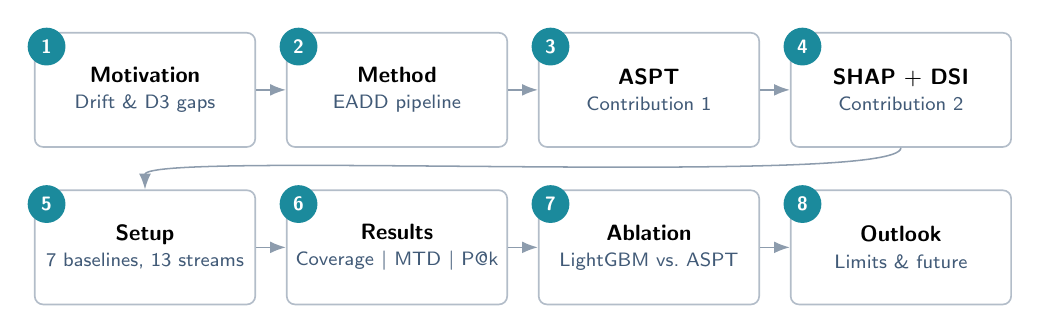
\begin{tikzpicture}[font=\footnotesize,
    stepbox/.style={draw=eaddSlate!40,fill=white,line width=0.6pt,rounded corners=3pt,
                  minimum width=2.8cm,minimum height=1.45cm,align=center,inner sep=3pt},
    num/.style={circle,fill=eaddTeal,text=white,font=\scriptsize\bfseries,
                inner sep=0pt,minimum size=4.8mm},
    arr/.style={-{Latex[length=2mm]},eaddSlate!60,line width=0.55pt}]
  \node[stepbox] (s1) at (0,0)    {\textbf{Motivation}\\{\scriptsize\color{eaddSlate}Drift \& D3 gaps}};
  \node[stepbox] (s2) at (3.2,0)  {\textbf{Method}\\{\scriptsize\color{eaddSlate}EADD pipeline}};
  \node[stepbox] (s3) at (6.4,0)  {\textbf{ASPT}\\{\scriptsize\color{eaddSlate}Contribution 1}};
  \node[stepbox] (s4) at (9.6,0)  {\textbf{SHAP $+$ DSI}\\{\scriptsize\color{eaddSlate}Contribution 2}};
  \node[stepbox] (s5) at (0,-2)   {\textbf{Setup}\\{\scriptsize\color{eaddSlate}7 baselines, 13 streams}};
  \node[stepbox] (s6) at (3.2,-2) {\textbf{Results}\\{\scriptsize\color{eaddSlate}Coverage \textbar{} MTD \textbar{} P@k}};
  \node[stepbox] (s7) at (6.4,-2) {\textbf{Ablation}\\{\scriptsize\color{eaddSlate}LightGBM vs.\ ASPT}};
  \node[stepbox] (s8) at (9.6,-2) {\textbf{Outlook}\\{\scriptsize\color{eaddSlate}Limits \& future}};
  \foreach \i/\n in {s1/1,s2/2,s3/3,s4/4,s5/5,s6/6,s7/7,s8/8}
    \node[num] at ([xshift=-1.25cm,yshift=0.55cm]\i.center) {\n};
  \draw[arr] (s1) -- (s2); \draw[arr] (s2) -- (s3); \draw[arr] (s3) -- (s4);
  \draw[arr] (s4.south) .. controls ([yshift=-0.5cm]s4.south) and ([yshift=0.5cm]s5.north) .. (s5.north);
  \draw[arr] (s5) -- (s6); \draw[arr] (s6) -- (s7); \draw[arr] (s7) -- (s8);
\end{tikzpicture}

\vspace{1.0em}
\centering\small\color{eaddSlate}
EADD answers \textcolor{eaddCoral}{\textbf{whether}}, \textcolor{eaddCoral}{\textbf{when}},
\textcolor{eaddCoral}{\textbf{which}}, and \textcolor{eaddCoral}{\textbf{how severe}}\,---\,in one pipeline.
\end{frame}

% ════════════════════ SECTION 1 ════════════════════
\sectionDivider{01}{The Problem}{Why production ML detectors miss the mark}

\setsec{01 \textbar{} THE PROBLEM}
\begin{frame}{Production ML models fail silently}
\vspace{0.3em}
\begin{columns}[T,onlytextwidth]
\column{0.56\textwidth}
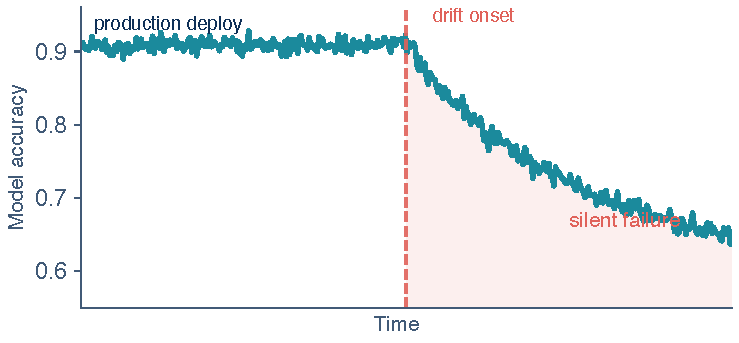
\includegraphics[width=\columnwidth]{drift_motivation.pdf}

\vspace{0.3em}
{\footnotesize \textbf{Distribution drift} silently degrades models.
Existing detectors raise a binary alarm; practitioners need:}

\smallskip
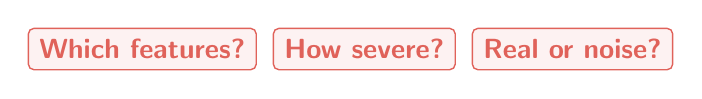
\begin{tikzpicture}[font=\footnotesize]
  \node[draw=eaddCoral,fill=eaddCoral!8,line width=0.5pt,rounded corners=2pt,
        inner sep=4pt,text=eaddCoral,font=\bfseries] (q1) {Which features?};
  \node[draw=eaddCoral,fill=eaddCoral!8,line width=0.5pt,rounded corners=2pt,
        inner sep=4pt,text=eaddCoral,font=\bfseries,right=2mm of q1] (q2) {How severe?};
  \node[draw=eaddCoral,fill=eaddCoral!8,line width=0.5pt,rounded corners=2pt,
        inner sep=4pt,text=eaddCoral,font=\bfseries,right=2mm of q2] (q3) {Real or noise?};
\end{tikzpicture}

\column{0.42\textwidth}
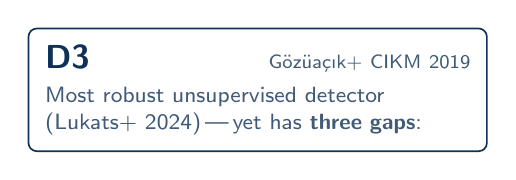
\begin{tikzpicture}
  \node[draw=eaddDeep,fill=white,line width=0.6pt,rounded corners=3pt,
        inner sep=6pt,text width=5.4cm,align=left,font=\footnotesize] (card) {%
    \textbf{\color{eaddDeep}\large D3} \hfill {\scriptsize\color{eaddSlate}Gözüaçık+ CIKM 2019}\\[3pt]
    {\color{eaddSlate}Most robust unsupervised detector
     (Lukats+ 2024)\,---\,yet has \textbf{three gaps}:}
  };
\end{tikzpicture}

\vspace{0.3em}
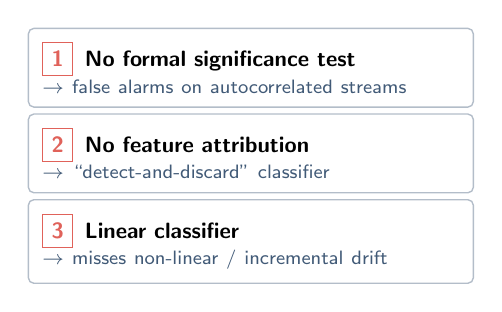
\begin{tikzpicture}[font=\footnotesize,
   gap/.style={draw=eaddSlate!40,fill=white,line width=0.5pt,rounded corners=2pt,
               text width=5.3cm,align=left,inner sep=5pt}]
  \node[gap] (g1) {%
    {\color{eaddCoral}\textbf{\fbox{1}}}\enspace \textbf{No formal significance test}\\
    {\scriptsize\color{eaddSlate}$\to$ false alarms on autocorrelated streams}};
  \node[gap,below=2pt of g1] (g2) {%
    {\color{eaddCoral}\textbf{\fbox{2}}}\enspace \textbf{No feature attribution}\\
    {\scriptsize\color{eaddSlate}$\to$ ``detect-and-discard'' classifier}};
  \node[gap,below=2pt of g2] (g3) {%
    {\color{eaddCoral}\textbf{\fbox{3}}}\enspace \textbf{Linear classifier}\\
    {\scriptsize\color{eaddSlate}$\to$ misses non-linear / incremental drift}};
\end{tikzpicture}
\end{columns}
\end{frame}

% ──────────────────── CAPABILITY MATRIX ────────────────────
\begin{frame}{Capability matrix \textbar{} the integration gap}
\vspace{0.2em}
\centering

\begin{tikzpicture}[font=\footnotesize,
    qcard/.style={draw,line width=0.8pt,rounded corners=3pt,
                  minimum width=3.6cm,minimum height=1.15cm,align=center,
                  inner sep=4pt}]
  \node[qcard,draw=eaddDeep,fill=eaddDeep!8]   (q1) at (-5.4,0)
    {\textbf{\color{eaddDeep}WHETHER}\\{\scriptsize\color{eaddSlate}Binary drift alarm}};
  \node[qcard,draw=eaddCoral,fill=eaddCoral!8] (q2) at (0,0)
    {\textbf{\color{eaddCoral}WHICH}\\{\scriptsize\color{eaddSlate}Feature attribution}};
  \node[qcard,draw=eaddAmber!85!black,fill=eaddAmber!18] (q3) at (5.4,0)
    {\textbf{\color{eaddAmber!70!black}HOW SEVERE}\\{\scriptsize\color{eaddSlate}Severity quantification}};
\end{tikzpicture}

\vspace{0.5em}
\centering
\renewcommand{\arraystretch}{1.25}
\setlength{\tabcolsep}{8pt}
{\footnotesize
\begin{tabular}{@{}>{\raggedright\arraybackslash}p{3.6cm} c c c c@{}}
\toprule
\rowcolor{eaddDeep!90}
\textcolor{white}{\textbf{Approach}} & \textcolor{white}{\textbf{Whether}} &
\textcolor{white}{\textbf{Which}}    & \textcolor{white}{\textbf{Severity}}  &
\textcolor{white}{\textbf{Streaming}} \\
\midrule
DDM / EDDM          & {\color{eaddLime}$\checkmark$} & {\color{eaddCoral}$\times$} & {\color{eaddCoral}$\times$} & {\color{eaddLime}$\checkmark$} \\
KS / KSWIN          & {\color{eaddLime}$\checkmark$} & {\color{eaddAmber!70!black}$\sim$} & {\color{eaddCoral}$\times$} & {\color{eaddLime}$\checkmark$} \\
D3                  & {\color{eaddLime}$\checkmark$} & {\color{eaddCoral}$\times$} & {\color{eaddCoral}$\times$} & {\color{eaddLime}$\checkmark$} \\
Vertex AI / Clarify & {\color{eaddLime}$\checkmark$} & {\color{eaddLime}$\checkmark$} & {\color{eaddAmber!70!black}$\sim$} & {\color{eaddCoral}$\times$} \\
TRIPODD / HDPD      & {\color{eaddLime}$\checkmark$} & {\color{eaddLime}$\checkmark$} & {\color{eaddCoral}$\times$} & {\color{eaddCoral}$\times$} \\
\midrule
\rowcolor{eaddTeal!85}
\textcolor{white}{\textbf{EADD (this work)}} &
\textcolor{white}{$\checkmark$} & \textcolor{white}{$\checkmark$} &
\textcolor{white}{$\checkmark$} & \textcolor{white}{$\checkmark$} \\
\bottomrule
\end{tabular}}
\end{frame}

% ──────────────────── CONTRIBUTIONS ────────────────────
\begin{frame}{Three contributions, one pipeline}
\vspace{0.3em}
\centering
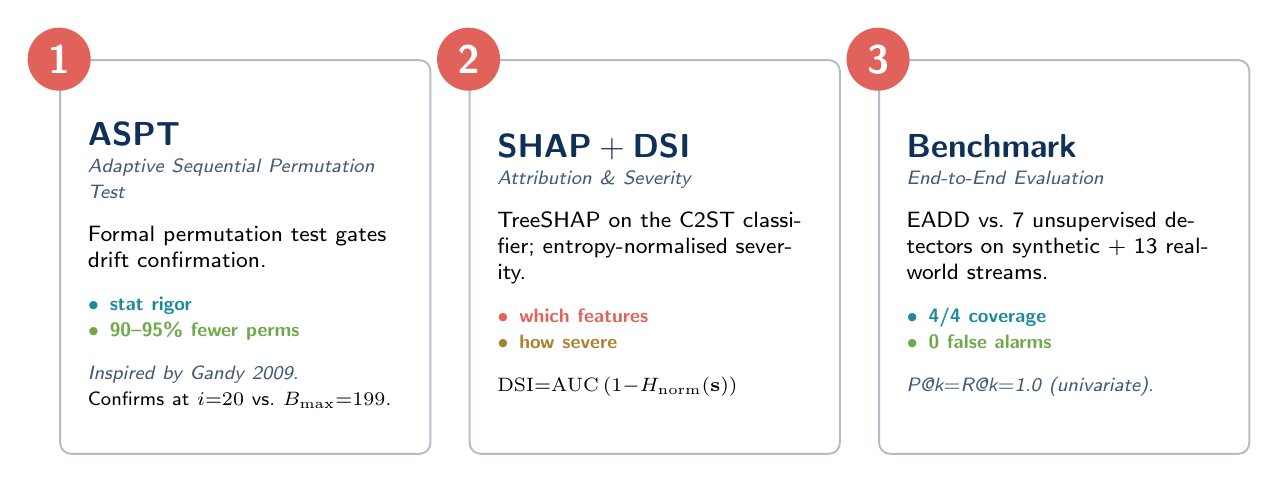
\begin{tikzpicture}[font=\footnotesize,
    card/.style={draw=eaddSlate!40,line width=0.7pt,rounded corners=4pt,
                 fill=white,minimum width=4.5cm,minimum height=5.0cm,
                 inner sep=10pt,align=left,text width=4.0cm,anchor=center},
    badge/.style={circle,fill=eaddCoral,text=white,font=\Large\bfseries,
                  inner sep=0pt,minimum size=8mm}]

  \node[card] (c1) at (-5.2,0) {%
    \vspace{0.6em}\\
    \textbf{\color{eaddDeep}\large ASPT}\\
    {\scriptsize\itshape\color{eaddSlate}Adaptive Sequential Permutation Test}\\[6pt]
    Formal permutation test gates drift confirmation.\\[6pt]
    {\scriptsize\color{eaddTeal}\textbf{$\bullet$\enspace stat rigor}}\\
    {\scriptsize\color{eaddLime}\textbf{$\bullet$\enspace 90--95\% fewer perms}}\\[6pt]
    {\scriptsize\color{eaddSlate}\itshape Inspired by Gandy 2009.}\\
    {\scriptsize Confirms at $i{=}20$ vs.\ $B_{\max}{=}199$.}};
  \node[card] (c2) at (0,0) {%
    \vspace{0.6em}\\
    \textbf{\color{eaddDeep}\large SHAP $+$ DSI}\\
    {\scriptsize\itshape\color{eaddSlate}Attribution \& Severity}\\[6pt]
    TreeSHAP on the C2ST classifier; entropy-normalised severity.\\[6pt]
    {\scriptsize\color{eaddCoral}\textbf{$\bullet$\enspace which features}}\\
    {\scriptsize\color{eaddAmber!70!black}\textbf{$\bullet$\enspace how severe}}\\[6pt]
    {\scriptsize $\mathrm{DSI}{=}\mathrm{AUC}\,(1{-}H_{\mathrm{norm}}(\mathbf{s}))$}};
  \node[card] (c3) at (5.2,0) {%
    \vspace{0.6em}\\
    \textbf{\color{eaddDeep}\large Benchmark}\\
    {\scriptsize\itshape\color{eaddSlate}End-to-End Evaluation}\\[6pt]
    EADD vs.\ 7 unsupervised detectors on synthetic $+$ 13 real-world streams.\\[6pt]
    {\scriptsize\color{eaddTeal}\textbf{$\bullet$\enspace 4/4 coverage}}\\
    {\scriptsize\color{eaddLime}\textbf{$\bullet$\enspace 0 false alarms}}\\[6pt]
    {\scriptsize\color{eaddSlate}\itshape P@k$=$R@k$=$1.0 (univariate).}};

  \node[badge] at (c1.north west) {1};
  \node[badge] at (c2.north west) {2};
  \node[badge] at (c3.north west) {3};
\end{tikzpicture}
\end{frame}

% ════════════════════ SECTION 2 ════════════════════
\sectionDivider{02}{The EADD Pipeline}{Four-step streaming detector}

\setsec{02 \textbar{} THE EADD PIPELINE}
\begin{frame}{End-to-end detection pipeline}
\vspace{-0.5em}
\centering
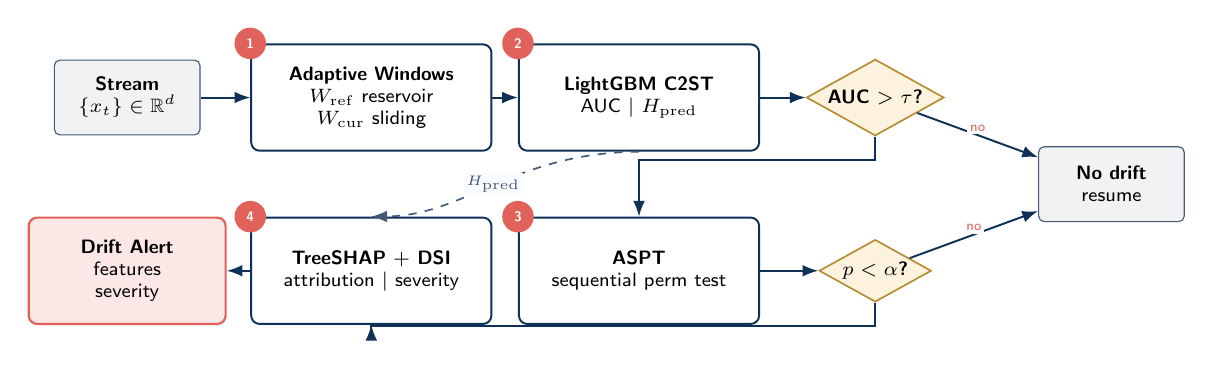
\begin{tikzpicture}[font=\scriptsize,
    proc/.style={draw=eaddDeep,fill=white,line width=0.7pt,rounded corners=3pt,
                 minimum width=3.05cm,minimum height=1.35cm,align=center,inner sep=3pt},
    dec/.style={diamond,draw=eaddAmber!75!black,fill=eaddAmber!18,line width=0.6pt,
                aspect=1.8,align=center,inner sep=1pt,font=\scriptsize\bfseries},
    term/.style={draw=eaddSlate,fill=eaddSlate!8,rounded corners=2pt,align=center,
                  minimum width=1.85cm,minimum height=0.95cm},
    alert/.style={draw=eaddCoral,fill=eaddCoral!15,line width=0.8pt,rounded corners=3pt,
                  align=center,minimum width=2.5cm,minimum height=1.35cm},
    arr/.style={-{Latex[length=2mm]},eaddDeep,line width=0.7pt},
    darr/.style={-{Latex[length=2mm]},eaddSlate,line width=0.6pt,dashed},
    num/.style={circle,fill=eaddCoral,text=white,font=\tiny\bfseries,
                inner sep=0pt,minimum size=4mm}]

  \node[term] (in) at (-6.5,0) {\textbf{Stream}\\$\{x_t\}\in\mathbb{R}^d$};
  \node[proc] (s1) at (-3.4,0) {\textbf{Adaptive Windows}\\$W_\mathrm{ref}$ reservoir\\$W_\mathrm{cur}$ sliding};
  \node[proc] (s2) at (0,0)    {\textbf{LightGBM C2ST}\\AUC \textbar{} $H_\mathrm{pred}$};
  \node[dec]  (d1) at (3.0,0)  {AUC $> \tau$?};
  \node[proc] (s3) at (0,-2.2) {\textbf{ASPT}\\sequential perm test};
  \node[dec]  (d2) at (3.0,-2.2) {$p < \alpha$?};
  \node[proc] (s4) at (-3.4,-2.2) {\textbf{TreeSHAP $+$ DSI}\\attribution \textbar{} severity};
  \node[alert] (out) at (-6.5,-2.2) {\textbf{Drift Alert}\\\scriptsize features\\\scriptsize severity};
  \node[term] (nd) at (6.0,-1.1) {\textbf{No drift}\\resume};

  \node[num] at (s1.north west) {1};
  \node[num] at (s2.north west) {2};
  \node[num] at (s3.north west) {3};
  \node[num] at (s4.north west) {4};

  \draw[arr] (in) -- (s1);
  \draw[arr] (s1) -- (s2);
  \draw[arr] (s2) -- (d1);
  \draw[arr] (d1) -- node[above,font=\tiny,text=eaddCoral,fill=eaddPaper,inner sep=1pt] {no} (nd);
  \draw[arr] (d1.south) -- ++(0,-0.3) -| (s3.north);
  \draw[arr] (s3) -- (d2);
  \draw[arr] (d2) -- node[above,font=\tiny,text=eaddCoral,fill=eaddPaper,inner sep=1pt] {no} (nd);
  \draw[arr] (d2.south) -- ++(0,-0.3) -| (s4.south);
  \draw[arr] (s4) -- (out);
  \draw[darr] (s2.south) .. controls (-1.6,-0.7) and (-2.2,-1.5) .. (s4.north)
    node[midway,fill=eaddPaper,font=\tiny,text=eaddSlate,inner sep=1pt] {$H_\mathrm{pred}$};
\end{tikzpicture}

\vspace{0.5em}
\centering{\footnotesize\color{eaddSlate}\itshape
Two-stage gate $\Rightarrow$ Type I error bound:
$\Pr(\mathrm{AUC}{>}\tau\mid H_0)\cdot\alpha \leq \alpha$.}
\end{frame}

% ════════════════════ ASPT ════════════════════
\setsec{02 \textbar{} CONTRIBUTION 1}
\begin{frame}{ASPT\,---\,Adaptive Sequential Permutation Test}
\begin{columns}[T,onlytextwidth]
\column{0.50\textwidth}
\textbf{Problem.} D3's fixed AUC threshold $\to$ false alarms on autocorrelated streams.

\smallskip
\textbf{Idea.} Permute labels iteratively; stop early once evidence is decisive.

\smallskip
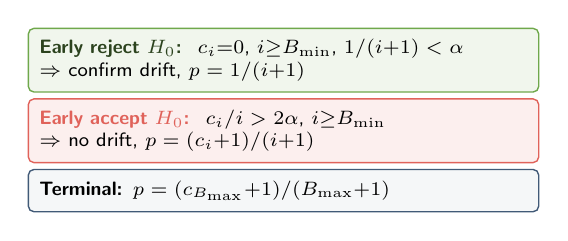
\begin{tikzpicture}[font=\scriptsize,
    box/.style={draw=eaddDeep,line width=0.5pt,rounded corners=2pt,
                fill=white,text width=6.2cm,inner sep=4pt,align=left}]
  \node[box,draw=eaddLime,fill=eaddLime!10] (r) {%
    \textbf{\color{eaddLime!40!black}Early reject $H_0$:}\;
    $c_i{=}0$, $i{\ge}B_{\min}$, $1/(i{+}1)<\alpha$\\
    $\Rightarrow$ confirm drift, $p=1/(i{+}1)$};
  \node[box,draw=eaddCoral,fill=eaddCoral!10,below=2pt of r] (a) {%
    \textbf{\color{eaddCoral}Early accept $H_0$:}\;
    $c_i/i > 2\alpha$, $i{\ge}B_{\min}$\\
    $\Rightarrow$ no drift, $p=(c_i{+}1)/(i{+}1)$};
  \node[box,draw=eaddSlate,fill=eaddSlate!5,below=2pt of a] (t) {%
    \textbf{Terminal:} $p=(c_{B_{\max}}{+}1)/(B_{\max}{+}1)$};
\end{tikzpicture}

\column{0.50\textwidth}
\centering
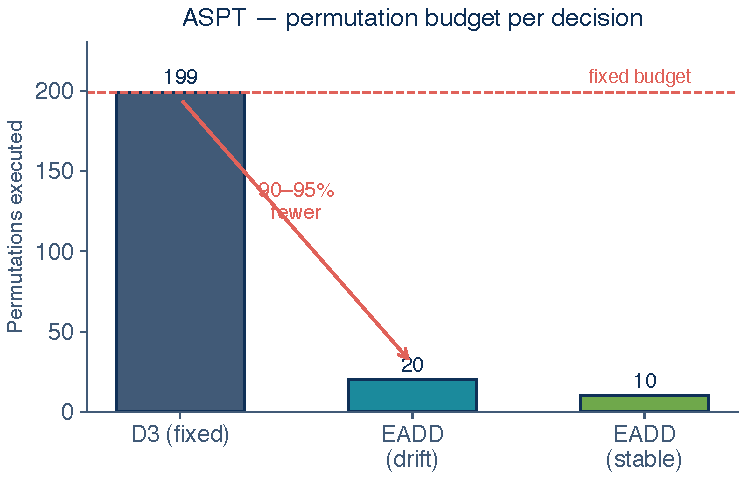
\includegraphics[width=\columnwidth]{aspt_savings.pdf}

\vspace{0.3em}
\centering
\colorbox{eaddTeal!18}{\small\textbf{\color{eaddDeep}90--95\% fewer permutations}
\textbar{} $\alpha$ preserved}
\end{columns}
\end{frame}

% ════════════════════ SHAP + DSI ════════════════════
\setsec{02 \textbar{} CONTRIBUTION 2}
\begin{frame}{SHAP attribution $+$ Drift Severity Index}
\begin{columns}[T,onlytextwidth]
\column{0.48\textwidth}
\textbf{TreeSHAP on the C2ST classifier} (which D3 discards).

\smallskip
\[
\bar\phi_j = \tfrac{1}{n}\sum_i |\phi_j^{(i)}|, \quad
s_j = \bar\phi_j \,/\, \textstyle\sum_k \bar\phi_k
\]

\textbf{Drift Severity Index.}
\[
\boxed{\;\mathrm{DSI}=\mathrm{AUC}\times(1-H_{\mathrm{norm}}(\mathbf{s}))\;}
\]
{\scriptsize $H_{\mathrm{norm}}(\mathbf{s})=-\sum_j s_j\log_2 s_j\,/\,\log_2 d \in[0,1]$\,---\,dimensionality-invariant.}

\column{0.52\textwidth}
\centering\textbf{\small Severity gradient \& prescription tiers}

\vspace{0.3em}
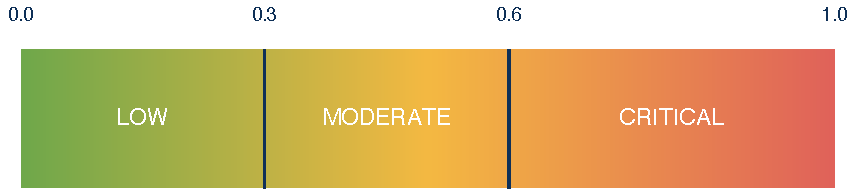
\includegraphics[width=0.96\columnwidth]{dsi_gradient.pdf}

\vspace{0.6em}
{\footnotesize
\begin{tabular}{@{}l p{4.6cm}@{}}
\toprule
\textbf{Tier} & \textbf{Recommended action} \\
\midrule
\textcolor{eaddLime!40!black}{\textbf{Low}} ($<\!0.3$)        & Diffuse shift $\to$ scheduled retrain \\
\textcolor{eaddAmber!70!black}{\textbf{Moderate}} (0.3--0.6) & Subset drift $\to$ audit shared source \\
\textcolor{eaddCoral}{\textbf{Critical}} ($>\!0.6$)           & Concentrated $\to$ audit pipeline \\
\bottomrule
\end{tabular}}

\vspace{0.2em}
{\scriptsize\itshape\color{eaddSlate}Heuristic tiers; require domain calibration.}
\end{columns}
\end{frame}

% ════════════════════ SECTION 3 ════════════════════
\sectionDivider{03}{Experiments \& Results}{What does EADD actually do?}

\setsec{03 \textbar{} EXPERIMENTS}
\begin{frame}{Experimental setup}
\centering
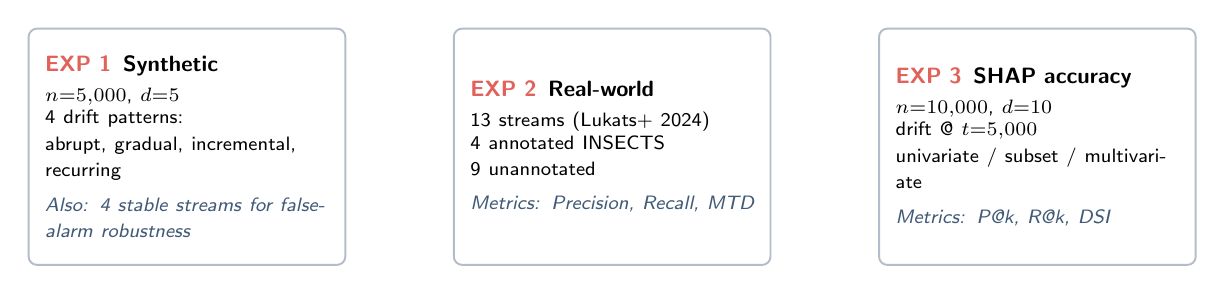
\begin{tikzpicture}[font=\footnotesize,
    card/.style={draw=eaddSlate!40,line width=0.7pt,rounded corners=3pt,
                 fill=white,minimum width=4.0cm,minimum height=3.0cm,
                 inner sep=6pt,align=left,text width=3.6cm}]
  \node[card] (e1) at (-5.4,0) {
    {\fontsize{8}{10}\selectfont\color{eaddCoral}\textbf{EXP 1}}\enspace\textbf{Synthetic}\\[3pt]
    {\scriptsize $n{=}5{,}000$, $d{=}5$\\
    4 drift patterns:\\abrupt, gradual, incremental, recurring}\\[3pt]
    {\scriptsize\color{eaddSlate}\itshape Also: 4 stable streams for false-alarm robustness}
  };
  \node[card] (e2) at (0,0) {
    {\fontsize{8}{10}\selectfont\color{eaddCoral}\textbf{EXP 2}}\enspace\textbf{Real-world}\\[3pt]
    {\scriptsize 13 streams (Lukats+ 2024)\\
    4 annotated INSECTS\\9 unannotated}\\[3pt]
    {\scriptsize\color{eaddSlate}\itshape Metrics: Precision, Recall, MTD}
  };
  \node[card] (e3) at (5.4,0) {
    {\fontsize{8}{10}\selectfont\color{eaddCoral}\textbf{EXP 3}}\enspace\textbf{SHAP accuracy}\\[3pt]
    {\scriptsize $n{=}10{,}000$, $d{=}10$\\
    drift @ $t{=}5{,}000$\\univariate / subset / multivariate}\\[3pt]
    {\scriptsize\color{eaddSlate}\itshape Metrics: P@k, R@k, DSI}
  };
\end{tikzpicture}

\vspace{0.6em}
\centering
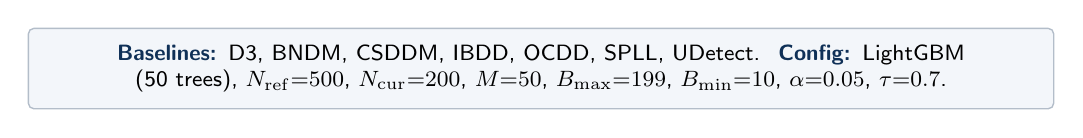
\begin{tikzpicture}[font=\footnotesize]
  \node[draw=eaddSlate!40,line width=0.5pt,rounded corners=2pt,fill=eaddMist,
        inner sep=6pt,text width=12.6cm,align=center] {%
    \textbf{\color{eaddDeep}Baselines:} D3, BNDM, CSDDM, IBDD, OCDD, SPLL, UDetect.\;
    \textbf{\color{eaddDeep}Config:} LightGBM (50 trees),
    $N_\mathrm{ref}{=}500$, $N_\mathrm{cur}{=}200$, $M{=}50$,
    $B_{\max}{=}199$, $B_{\min}{=}10$, $\alpha{=}0.05$, $\tau{=}0.7$.};
\end{tikzpicture}
\end{frame}

% ──────────────────── HEADLINE STATS ────────────────────
\setsec{03 \textbar{} HEADLINE}
\begin{frame}{Headline results}
\vspace{0.4em}
\centering
\statTile{4/4}{synthetic\\coverage}{eaddTeal}\hfill
\statTile{0}{false alarms\\on stable streams}{eaddLime}\hfill
\statTile{8.3$\boldsymbol{\times}$}{faster MTD\\vs.\ D3 (incremental)}{eaddCoral}\hfill
\statTile{1.00}{P@k$=$R@k\\(univariate SHAP)}{eaddAmber!75!black}

\vspace{1.0em}
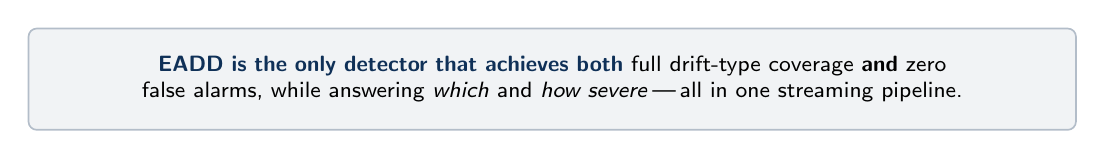
\begin{tikzpicture}[font=\footnotesize]
  \node[draw=eaddSlate!40,line width=0.6pt,rounded corners=3pt,fill=eaddDeep!6,
        inner sep=10pt,text width=12.6cm,align=center] {%
    \textbf{\color{eaddDeep}EADD is the only detector that achieves both}
    full drift-type coverage \textbf{and} zero false alarms,
    while answering \textit{which} and \textit{how severe}\,---\,all in one streaming pipeline.};
\end{tikzpicture}

\vspace{0.6em}
{\scriptsize\color{eaddSlate}Mann--Whitney U vs.\ D3 on autocorrelated streams: $p=0.0101$ ($\tau{=}0.6$).
Source data: \texttt{experiments/results/}.}
\end{frame}

% ──────────────────── RESULT 1 ────────────────────
\setsec{03 \textbar{} RESULT 1}
\begin{frame}{Synthetic coverage \& false alarms}
\vspace{-0.4em}
\centering
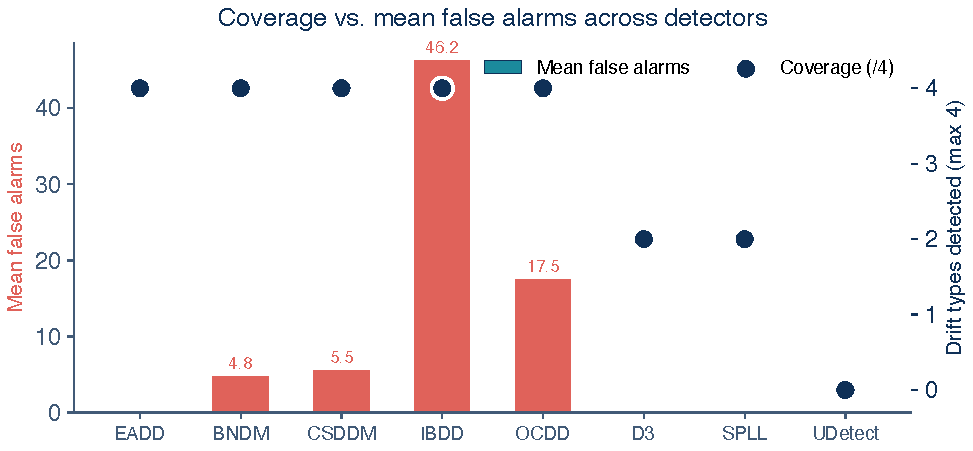
\includegraphics[width=0.78\textwidth]{coverage_falsealarms.pdf}

\vspace{0.2em}

\begin{tikzpicture}[font=\footnotesize]
  \node[fill=eaddTeal,rounded corners=3pt,text=white,inner sep=5pt,
        text width=12.6cm,align=center] {%
    \textbf{EADD: 4/4 coverage AND 0 false alarms.}
    BNDM/CSDDM/IBDD/OCDD also hit 4/4 but pay heavy FA cost;
    D3/SPLL keep 0 FA only by missing half the drift types.};
\end{tikzpicture}
\end{frame}

% ──────────────────── RESULT 2 ────────────────────
\setsec{03 \textbar{} RESULT 2}
\begin{frame}{INSECTS\,---\,faster detection on incremental drift}
\vspace{-0.4em}
\centering
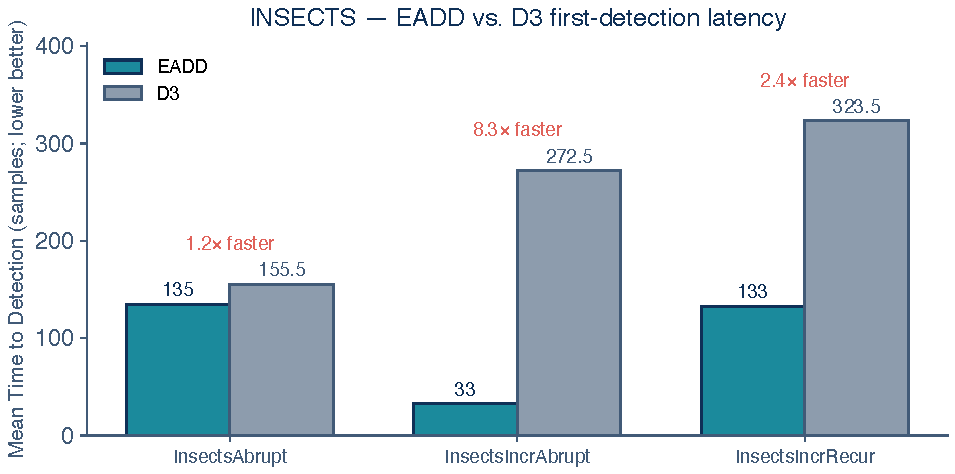
\includegraphics[width=0.66\textwidth]{mtd_insects.pdf}

\vspace{0.2em}
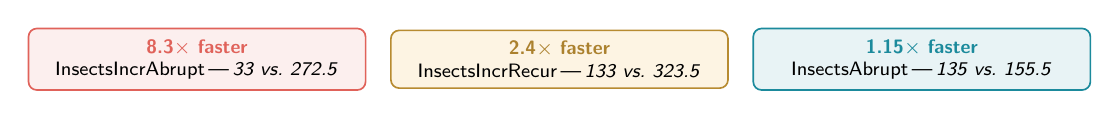
\begin{tikzpicture}[font=\scriptsize,
   tile/.style={rounded corners=3pt,line width=0.6pt,inner sep=4pt,
                text width=4.0cm,align=center}]
  \node[tile,draw=eaddCoral,fill=eaddCoral!10] (a)
    {\textbf{\color{eaddCoral}8.3$\times$ faster}\\InsectsIncrAbrupt\,---\,\textit{33 vs.\ 272.5}};
  \node[tile,draw=eaddAmber!75!black,fill=eaddAmber!15,right=0.3cm of a] (b)
    {\textbf{\color{eaddAmber!70!black}2.4$\times$ faster}\\InsectsIncrRecur\,---\,\textit{133 vs.\ 323.5}};
  \node[tile,draw=eaddTeal,fill=eaddTeal!10,right=0.3cm of b] (c)
    {\textbf{\color{eaddTeal}1.15$\times$ faster}\\InsectsAbrupt\,---\,\textit{135 vs.\ 155.5}};
\end{tikzpicture}
\end{frame}

% ──────────────────── RESULT 3 ────────────────────
\setsec{03 \textbar{} RESULT 3}
\begin{frame}{SHAP attribution\,---\,P@k $=$ R@k $=$ 1.0}
\vspace{-0.4em}
\centering
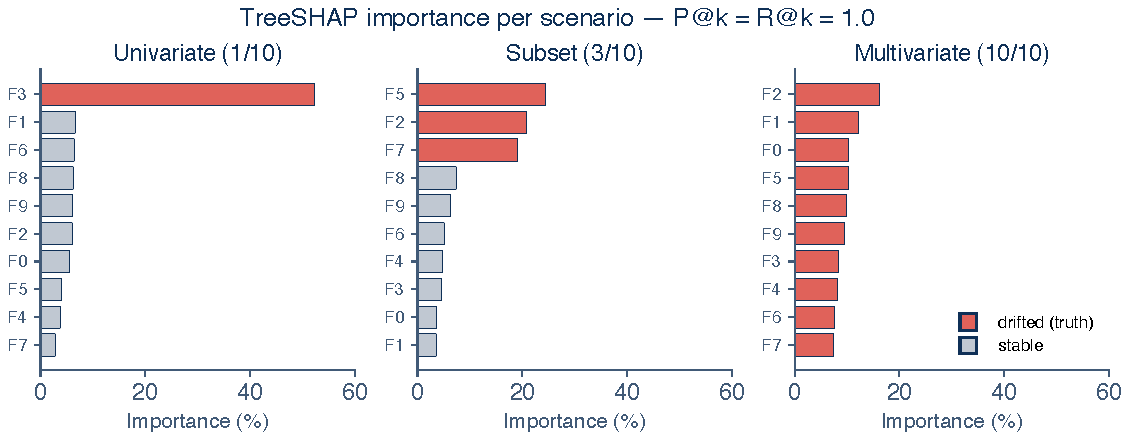
\includegraphics[width=0.78\textwidth]{shap_per_scenario.pdf}

\vspace{0.2em}
\begin{columns}[T,onlytextwidth]
\column{0.50\textwidth}
{\footnotesize
\setlength{\tabcolsep}{4pt}
\begin{tabular}{@{}l c c c@{}}
\toprule
\textbf{Scenario} & \textbf{AUC} & \textbf{Top feat.} & \textbf{DSI} \\
\midrule
Univariate (1/10)    & 0.784 & \textbf{F3} (52.3\%) & 0.193 \\
Subset (3/10)        & 0.809 & F5 (24.5\%)          & 0.096 \\
Multivariate (10/10) & 0.806 & F2 (14.6\%)          & 0.016 \\
\bottomrule
\end{tabular}}

\column{0.48\textwidth}
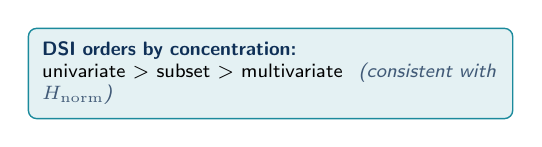
\begin{tikzpicture}[font=\scriptsize]
\node[fill=eaddTeal!12,draw=eaddTeal,line width=0.5pt,rounded corners=3pt,
      inner sep=5pt,text width=5.8cm,align=left] {%
\textbf{\color{eaddDeep}DSI orders by concentration:}\\
univariate $>$ subset $>$ multivariate
\;{\scriptsize\color{eaddSlate}\itshape\,(consistent with $H_{\mathrm{norm}}$)}};
\end{tikzpicture}
\end{columns}
\end{frame}

% ──────────────────── RESULT 4 ────────────────────
\setsec{03 \textbar{} RESULT 4}
\begin{frame}{False-alarm robustness on stable streams}
\vspace{-0.4em}
\centering
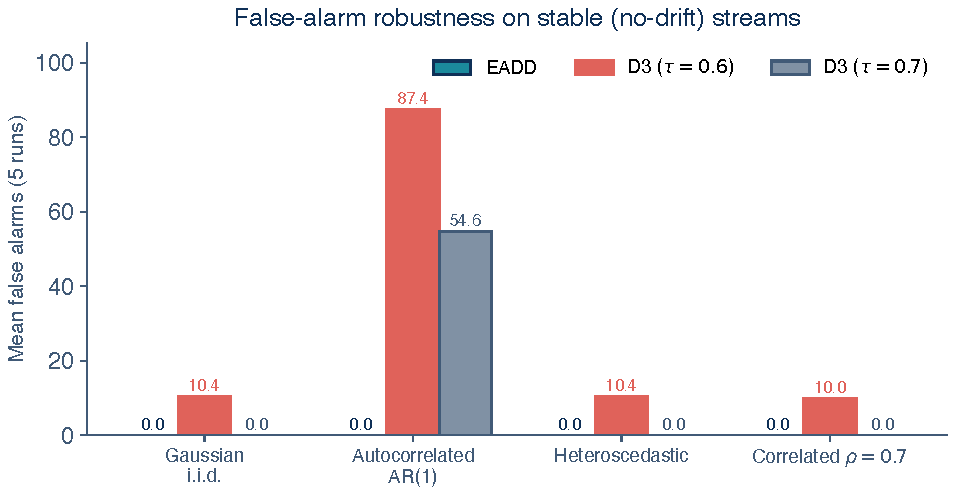
\includegraphics[width=0.74\textwidth]{false_alarms_stable.pdf}

\vspace{0.2em}
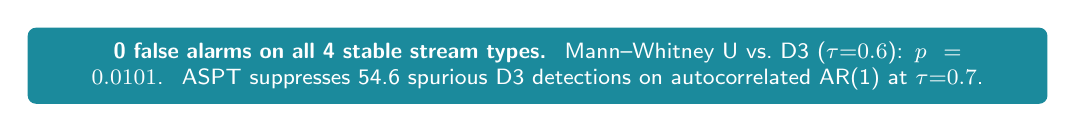
\begin{tikzpicture}[font=\footnotesize]
  \node[fill=eaddTeal,rounded corners=3pt,text=white,inner sep=5pt,
        text width=12.6cm,align=center] {%
    \textbf{0 false alarms on all 4 stable stream types.}\;
    Mann--Whitney U vs.\ D3 ($\tau{=}0.6$): \textbf{$p=0.0101$}.\;
    ASPT suppresses 54.6 spurious D3 detections on autocorrelated AR(1) at $\tau{=}0.7$.};
\end{tikzpicture}
\end{frame}

% ════════════════════ SECTION 4 ════════════════════
\sectionDivider{04}{Ablation \& Cost}{Where does the gain come from?}

\setsec{04 \textbar{} ABLATION}
\begin{frame}{Where does the gain come from?}
\begin{columns}[T,onlytextwidth]
\column{0.55\textwidth}
\centering
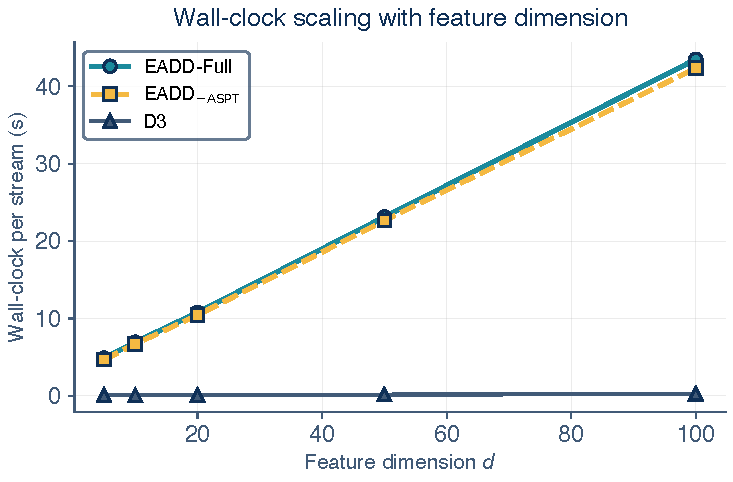
\includegraphics[width=\columnwidth]{runtime_scaling_d.pdf}

\column{0.45\textwidth}
\vspace{0.4em}
\textbf{\color{eaddDeep}Decomposing the gain}

\smallskip
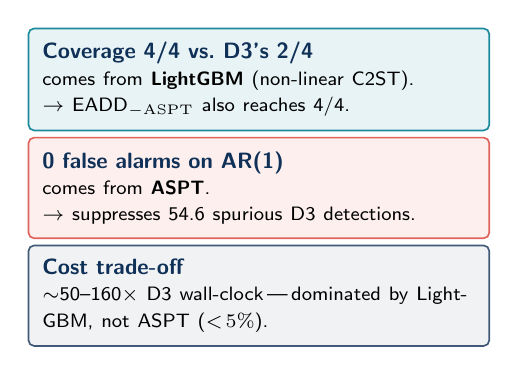
\begin{tikzpicture}[font=\footnotesize,
  card/.style={draw,line width=0.6pt,rounded corners=2pt,
               text width=5.5cm,align=left,inner sep=5pt}]
  \node[card,draw=eaddTeal,fill=eaddTeal!10] (a) {%
    \textbf{\color{eaddDeep}Coverage 4/4 vs.\ D3's 2/4}\\
    {\scriptsize comes from \textbf{LightGBM} (non-linear C2ST).}\\
    {\scriptsize $\to$ EADD$_{-\mathrm{ASPT}}$ also reaches 4/4.}};
  \node[card,draw=eaddCoral,fill=eaddCoral!10,below=2pt of a] (b) {%
    \textbf{\color{eaddDeep}0 false alarms on AR(1)}\\
    {\scriptsize comes from \textbf{ASPT}.}\\
    {\scriptsize $\to$ suppresses 54.6 spurious D3 detections.}};
  \node[card,draw=eaddSlate,fill=eaddSlate!8,below=2pt of b] (c) {%
    \textbf{\color{eaddDeep}Cost trade-off}\\
    {\scriptsize $\sim$50--160$\times$ D3 wall-clock\,---\,dominated by LightGBM, not ASPT ($<\!5\%$).}};
\end{tikzpicture}
\end{columns}
\end{frame}

% ════════════════════ SECTION 5 ════════════════════
\sectionDivider{05}{Limits \& Outlook}{What EADD cannot answer\,---\,yet}

\setsec{05 \textbar{} LIMITS}
\begin{frame}{Limitations \& future work}
\begin{columns}[T,onlytextwidth]
\column{0.50\textwidth}
\textbf{\color{eaddCoral}Limitations}
\begin{itemize}\setlength\itemsep{2pt}\footnotesize
  \item Wall-clock $\sim$50--160$\times$ D3\,---\,LightGBM retrains every $M{=}50$ steps.
  \item \textbf{Multiple testing over time:} $\sim$600 tests/30K samples;
        Bonferroni $\alpha'{\approx}8.3{\times}10^{-5}$ below ASPT's $1/(B_{\max}{+}1){=}0.005$ floor.\\
        {\scriptsize\itshape Zero-FA result empirical, not theoretically guaranteed.}
  \item DSI tier boundaries heuristic; never triggered above LOW in experiments.
  \item SHAP attributions correlational, not causal.
  \item No isolation of reservoir sampling vs.\ window config contributions.
\end{itemize}

\column{0.50\textwidth}
\textbf{\color{eaddTeal}Future work}
\begin{itemize}\setlength\itemsep{2pt}\footnotesize
  \item Anytime-valid \textbf{e-values} for streaming FWER control.
  \item \textbf{Causal} attribution (Budhathoki+ AISTATS 2021).
  \item Multi-domain \textbf{DSI calibration} to ground tier boundaries empirically.
  \item Adversarial robustness of discriminative drift detectors.
  \item Per-feature operating curves under correlation $\to$ feature-group SHAP.
\end{itemize}

\vspace{0.4em}
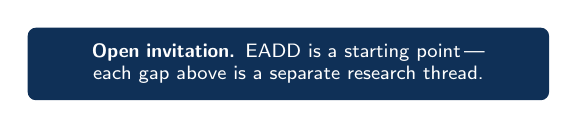
\begin{tikzpicture}[font=\scriptsize]
  \node[fill=eaddDeep,rounded corners=3pt,text=white,inner sep=6pt,
        text width=6.2cm,align=center,font=\scriptsize] {%
    \textbf{Open invitation.} EADD is a starting point\,---\,each gap above is a separate research thread.};
\end{tikzpicture}
\end{columns}
\end{frame}

% ════════════════════ CONCLUSION ════════════════════
\setsec{CONCLUSION}
\begin{frame}{Conclusion}
\vspace{0.3em}
\centering

\begin{tikzpicture}[font=\footnotesize,
    pill/.style={fill=eaddDeep,text=white,rounded corners=10pt,
                 inner xsep=12pt,inner ysep=6pt,font=\bfseries}]
  \node[pill] {EADD answers \textcolor{eaddAmber}{WHETHER},
               \textcolor{eaddAmber}{WHEN},
               \textcolor{eaddAmber}{WHICH}, and
               \textcolor{eaddAmber}{HOW SEVERE}\,---\,in one pipeline.};
\end{tikzpicture}

\vspace{0.8em}
\centering
\statTile{4/4}{coverage}{eaddTeal}\hfill
\statTile{0}{false alarms}{eaddLime}\hfill
\statTile{8.3$\boldsymbol{\times}$}{faster MTD}{eaddCoral}\hfill
\statTile{1.00}{SHAP P@k}{eaddAmber!75!black}

\vspace{0.8em}
\begin{columns}[T,onlytextwidth]
\column{0.50\textwidth}
\textbf{\color{eaddDeep}What we built}
\begin{itemize}\setlength\itemsep{1pt}\footnotesize
  \item ASPT $+$ $H_{\mathrm{pred}}$\,---\,rigorous confirmation, 90--95\% perm savings.
  \item SHAP $+$ DSI\,---\,feature-level diagnosis $+$ severity.
  \item Benchmark vs.\ 7 unsupervised detectors.
\end{itemize}

\column{0.50\textwidth}
\textbf{\color{eaddDeep}What it gives MLOps}
\begin{itemize}\setlength\itemsep{1pt}\footnotesize
  \item Reliable alarms on autocorrelated production streams.
  \item Actionable diagnoses, not just binary flags.
  \item Severity-tiered prescriptions for response.
\end{itemize}
\end{columns}
\end{frame}

% ════════════════════ THANK YOU ════════════════════
\begin{frame}[plain,noframenumbering]

\begin{tikzpicture}[remember picture,overlay]
  \fill[eaddDeep] (current page.south west) rectangle (current page.north east);
  \fill[eaddTeal,opacity=0.45]
    (current page.south east) -- ([xshift=-7.5cm]current page.south east)
    -- ([xshift=-3.5cm]current page.north east) -- (current page.north east) -- cycle;
  \foreach \i in {0,1,2,3,4}{
    \draw[eaddAmber,opacity={0.10+0.02*\i},line width=0.6pt]
      ([xshift=2cm+0.4*\i cm,yshift=2cm+0.3*\i cm]current page.south west)
      circle ({1.0cm+0.4*\i cm});
  }
  \node[anchor=center,text=white,font=\fontsize{56}{60}\bfseries]
    at ([yshift=0.8cm]current page.center) {Thank you.};
  \node[anchor=center,text=eaddAmber,font=\Large\itshape]
    at ([yshift=-0.5cm]current page.center) {Questions \& discussion welcome.};
  \node[anchor=center,text=white,font=\small]
    at ([yshift=-1.8cm]current page.center)
    {\textbf{Nusrat Begum} \textbar{} \texttt{nusrat.beg@student.mahidol.ac.th}};
  \node[anchor=south,text=white!60,font=\scriptsize]
    at ([yshift=0.6cm]current page.south) {Code + paper available at the project repository.};
\end{tikzpicture}
\end{frame}

% ════════════════════ APPENDIX ════════════════════
\appendix
\setsec{APPENDIX}

\begin{frame}{Backup \textbar{} runtime scaling vs.\ window size}
\begin{columns}[T,onlytextwidth]
\column{0.58\textwidth}
\centering
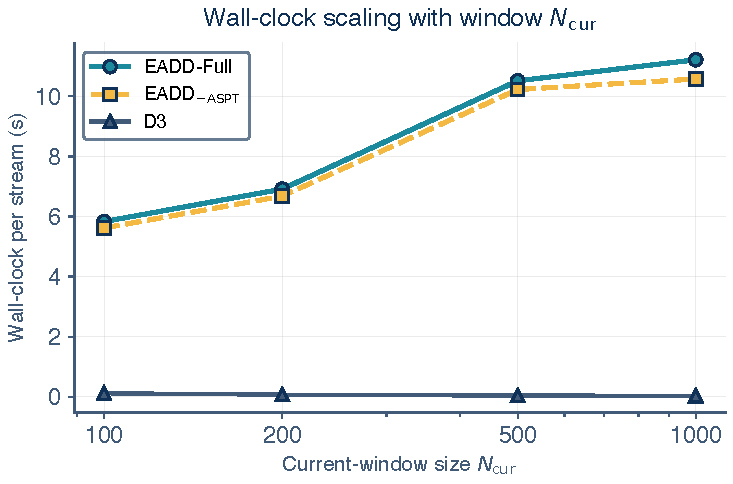
\includegraphics[width=\columnwidth]{runtime_scaling_n.pdf}

\column{0.42\textwidth}
\vspace{0.6em}
\begin{itemize}\footnotesize\setlength\itemsep{3pt}
  \item $N_\mathrm{cur}{=}200{\to}1000$: EADD time grows only \textbf{1.6$\times$}.
  \item LightGBM cost sub-linear in $N$, near-linear in $d$.
  \item ASPT overhead $<\!5\%$ across window sizes.
\end{itemize}

\vspace{0.5em}
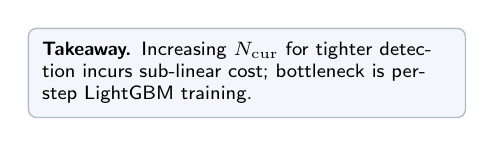
\begin{tikzpicture}[font=\footnotesize]
  \node[fill=eaddMist,draw=eaddSlate!40,line width=0.5pt,rounded corners=3pt,
        inner sep=5pt,text width=5.2cm,align=left,font=\scriptsize] {%
    \textbf{Takeaway.} Increasing $N_\mathrm{cur}$ for tighter detection incurs sub-linear cost;
    bottleneck is per-step LightGBM training.};
\end{tikzpicture}
\end{columns}
\end{frame}

\begin{frame}{Backup \textbar{} correlated features ($d{=}10$)}
\begin{columns}[T,onlytextwidth]
\column{0.55\textwidth}
\centering
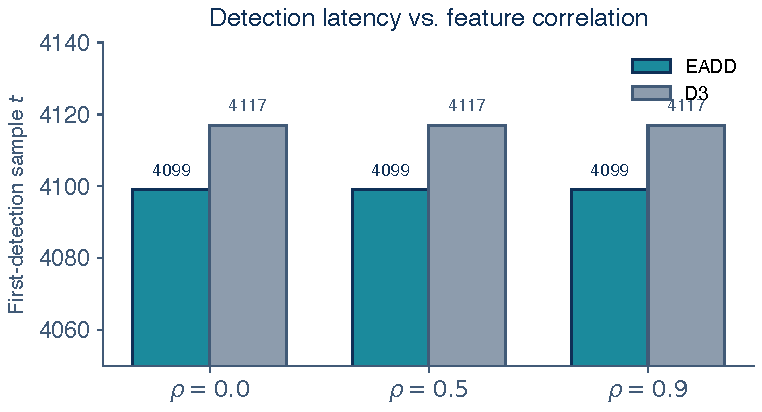
\includegraphics[width=\columnwidth]{correlated_features.pdf}

\column{0.45\textwidth}
\vspace{0.8em}
\begin{itemize}\footnotesize\setlength\itemsep{4pt}
  \item Cholesky-mixed Gaussian; $+2\sigma$ shift in 3 features at $t{=}4000$.
  \item EADD detection robust to correlation; stable correlated streams give \textbf{0 FA}.
  \item SHAP under correlation $\to$ interpret at \textbf{feature-group} granularity.
\end{itemize}
\end{columns}
\end{frame}

\begin{frame}{Backup \textbar{} incremental-drift timeline}
\centering
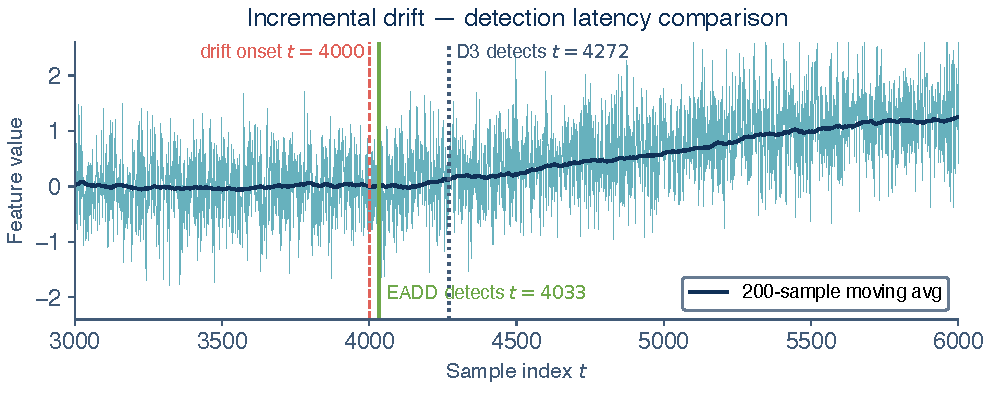
\includegraphics[width=0.86\textwidth]{insects_timeseries.pdf}

\vspace{0.3em}
{\footnotesize\color{eaddSlate}\itshape Illustrative INSECTS-style trace; EADD detects within $\sim$33 samples vs.\ D3's $\sim$272.5.}
\end{frame}

\end{document}
